\documentclass[14pt,a4paper,oneside]{article}

\usepackage[utf8]{inputenc}   


\usepackage{amsmath,amsthm,amssymb,appendix,bm,mathrsfs,ctex,geometry,tcolorbox,fancyhdr,tikz,esint,appendix}


%% GB/T 7714 宏包 ---- 引文格式
\usepackage[sort&compress]{gbt7714}
\bibliographystyle{gbt7714-numerical}



\numberwithin{equation}{section}             %%%%%% 公式编号




\geometry{left=1.7cm, right=1.7cm, top=2.54cm, bottom=2.54cm}    %%%%% 页面尺寸
\linespread{1.5}                             %%%%% 行距1.5倍
\pagestyle{fancy}



%%    设置页眉页脚
\fancyhf{}
\renewcommand{\headrulewidth}{0.15mm}
\fancyhead[C]{读书笔记}                   %%%%%% 页眉
\fancyfoot[C]{\thepage}                      %%%%%% 页脚 页码
\setlength{\headheight}{15pt}


%%   设置各种链接颜色为黑色
\usepackage[colorlinks,
            linkcolor=black,
            anchorcolor=black,
            citecolor=black,
            urlcolor=blue
            ]{hyperref}



%%   例子编号
\newcounter{example}
\counterwithin{example}{subsection}
\newcommand{\examplename}{Example}
\newcommand{\exampleTitle}[1]{%
\textbf{\refstepcounter{example}\examplename\theexample:#1}\par}


%%  插入图片配置
\usepackage{graphicx,subfigure}
\usepackage[]{caption2} %新增调用的宏包
\numberwithin{figure}{section}               %%%%%% 图片编号按节

\graphicspath{ {./Figure/} }            %%%%% 设置图片文件所在目录
\DeclareGraphicsExtensions{.pdf,.svg,.jpeg,.png,.jpg}     %%%%% 支持图片格式


%%    支持tikz作图
\usepackage{tikz}
\usetikzlibrary{backgrounds,arrows}


\usepackage{pgfplots}
\pgfplotsset{compat=1.15}
\usepackage{mathrsfs}


\title{\textbf{读书笔记 Part 1\\Quantum Field Theory and the Standard Model}}                           %%%%% 标题
\author{骆禹天}                                           %%%%% 作者
\date{2024/**/**}                                        %%%%%% 日期

%%   定义一些数学格式
\newtheorem{theorem}{定理}[]
\newtheorem{definition}[theorem]{定义}
\newtheorem{lemma}[theorem]{引理}
\newtheorem{corollary}[theorem]{推论}
\newtheorem{example}[theorem]{例}
\newtheorem{proposition}[theorem]{命题}
\renewcommand{\abstractname}{\Large\textbf{摘要}}




%------------------------- 开始文档  -------------------------%



\begin{document}

\pagenumbering{Roman}         %%%%% 目录前页码统计按罗马数字

\maketitle

\setcounter{page}{1}          %%%%% 标题开始统计页数

%------------------------- 目录  ------------------------------%

\tableofcontents              %%%%% 插入目录

\newpage
\setcounter{page}{1}          %%%%% 目录后重新统计页数


\pagenumbering{arabic}        %%%%% 目录后统计页码为阿拉伯数字



%%%%%%%%%%%%%%%%%%%% 开始第一节  %%%%%%%%%%%%%%%%%%%%%



\section{Microscopic theory of radiation}

\subsection{Blackbody radiation}

1900 年，没有人能给出热物体的辐射光谱的明确解释。当时一个合理方法是应用均分定理，这意味着处于热平衡物体的能量应该在所有可能的模式中平均分配。对于热气体，该定理预测了热速度的麦克斯韦-玻尔兹曼分布，这与数据非常吻合。然而当应用于热物体的光谱时，均分定理会导致奇怪的结果。

黑体, 指固定温度下一个处于热平衡的热箱。传统上，尺寸为 L 的盒子支持具有角频率的驻电磁波
\begin{equation}
    \omega_n=\frac{2\pi}{L}|\vec{n}|c
    \label{eq:1.1}
\end{equation}
其中, 3维整数向量 n, c 是光速。 

1900 年前，物理学家相信每种模式下的能量可以任意多或少。根据（经典）均分定理，黑体应该在所有模式下均等地发光，并且强度随着相空间的微分体积而增长：
\begin{equation}
    I(\omega)\equiv\frac{1}{V}\frac{d}{d\omega}E(\omega)=\text{const}\times c^{-3}\omega^2k_B T\quad\text{(classical)}
    \label{eq:1.2}
\end{equation}

\begin{figure}[h]
    \centering
    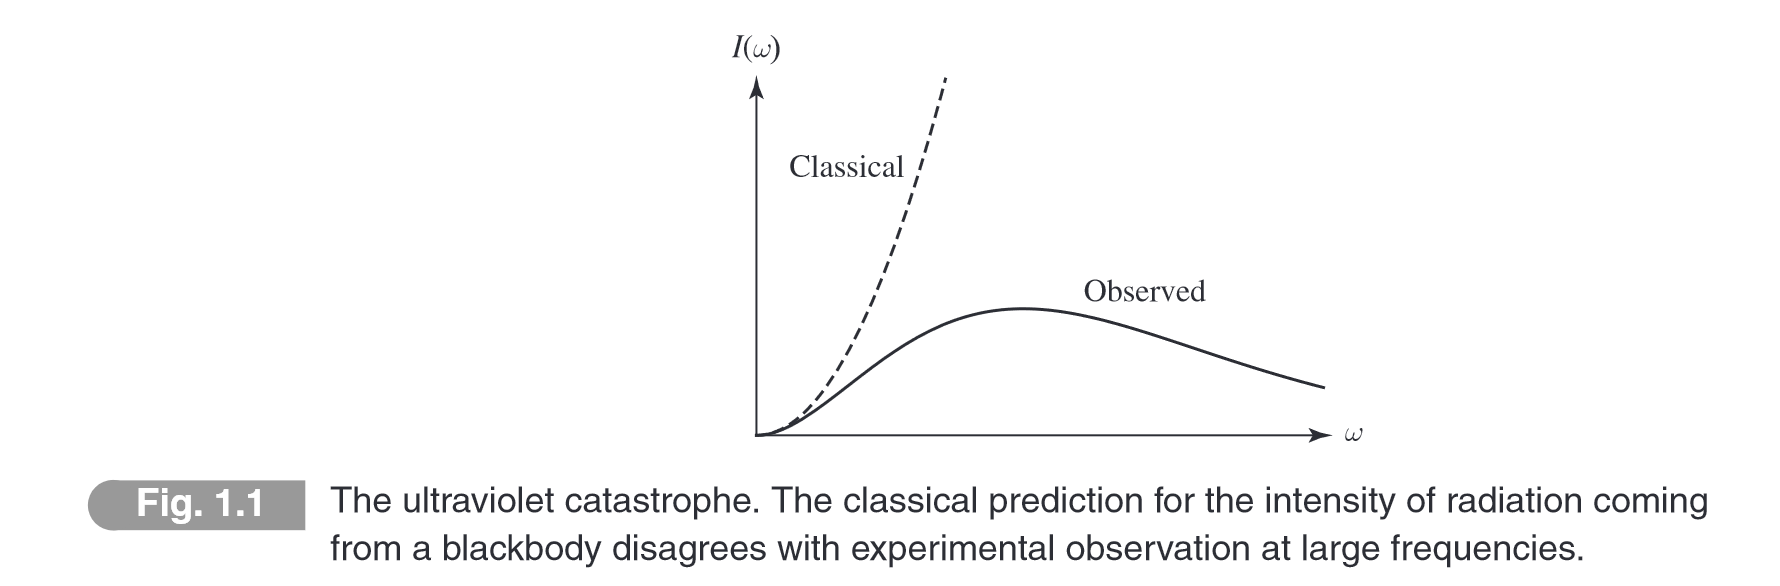
\includegraphics[width=0.9\textwidth]{p1_1.png}
    \label{p1.1}
\end{figure}

经典光谱意味着每单位频率发射的辐射量应随频率而增加，这种结果称为紫外线灾难。然而实验上，该分布更接近麦克斯韦-玻尔兹曼分布，在某个有限 $\omega$  处达峰值，如图 \ref{p1.1}。显然，均分定理不适用于黑体辐射。

由于观测结果与经典预测相悖，普朗克假设空腔中每种电磁模式的能量以频率为单位进行量化：
\begin{equation}
    E_n=\hbar\omega_n=\frac{2\pi}{L}\hbar|\vec n|=|\vec p_n|
    \label{eq:1.3}
\end{equation}
其中 $h$ 是普朗克常数，$\hbar \equiv h/2π$ 。阿尔伯特·爱因斯坦后来解释这暗示光是由粒子组成的。注意，若激励是粒子，那么它们是无质量的：
\begin{equation}
    m_n^2=E_n^2-|\vec{p}_n|^2=0
    \label{eq:1.4}
\end{equation}

按照普朗克和爱因斯坦, 光实际上是无质量光子的集合。这个假设有许多简单而直接的实验结果：量子化光解决了黑体悖论；具有能量的光会产生光电效应；具有动量的光会导致康普顿散射。

根据普朗克能量假说，频率 $\omega _n$ 的每种模式可被激发整数 $j$ 次，每个模式下给出能量 $jE_n = j(\hbar \omega _n)$. 在该模式中找到那么多能量的概率与在任何事物中找到能量的概率相同，与玻尔兹曼权重 $\exp(-energy/k_BT )$ 成正比。因此，各模式下的能量期望值为
\begin{equation}
    \langle E_n\rangle=\frac{\sum_{j=0}^\infty(jE_n)e^{-jE_n\beta}}{\sum_{j=0}^\infty e^{-jE_n\beta}}=\frac{-\frac{d}{d\beta}\frac{1}{1-e^{-\hbar\omega_n\beta}}}{\frac{1}{1-e^{-\hbar\omega_n\beta}}}=\frac{\hbar\omega_n}{e^{\hbar\omega_n\beta}-1}
    \label{eq:1.5}
\end{equation}
其中 $\beta = 1/k_BT$.

现在取连续极限，$L \rightarrow  \infty$。在此限制下，总和变成积分，黑体中频率 $\omega$ 的平均总能量为
\begin{equation}
    \begin{aligned}E(\omega)&=\int^{\omega}d^{3}\vec{n}\frac{\hbar\omega_{n}}{e^{\hbar\omega_{n}\beta}-1}=\int_{-1}^{1}d\cos\theta\int_{0}^{2\pi}d\phi\int_{0}^{\omega}d|\vec{n}|\frac{|\vec{n}|^{2}\hbar\omega_{n}}{e^{\hbar\omega_{n}\beta}-1}\\&=4\pi\hbar\frac{L^3}{8\pi^3}\int_0^\omega d\omega^{\prime}\frac{\omega^{\prime3}}{e^{\hbar\omega^{\prime}\beta}-1}.\end{aligned}
    \label{eq:1.6}
\end{equation}

因此，光的强度作为频率的函数为（为光的两个偏振添加因子 2）
\begin{equation}
    I(\omega)=\frac1V\frac{dE(\omega)}{d\omega}=\frac\hbar{\pi^2}\frac{\omega^3}{e^{\hbar\omega\beta}-1}.
    \label{eq:1.7}
\end{equation}
这正是普朗克在1900年展示的函数形式与实验的正确匹配。

这与量子场论有什么关系？

为了使这个使用平衡统计力学的推导有意义，光必须能够平衡。例如，如果我们用单色光加热一个盒子，最终所有频率都必须被激发。然而，如果不同的频率是不同的粒子，则平衡必须涉及一种粒子变成另一种粒子。因此，粒子必须被创造和毁灭。量子场论告诉我们这是如何发生的。

\subsection{Einstein coefficients}

量化光的产生的一种直接方法是通过自发发射系数。这是受激原子发光的速率。

1916年，爱因斯坦基于热平衡的存在，提出了发射和吸收之间关系的简单证明:

假设我们有一个充满能级为 $E_1$ 和 $E_2$ 的原子的空腔。假设有 $n_1$ 个 $E_1$ 原子和 $n_2$ 个 $E_2$ 原子，并令 $\hbar \omega = E_2 - E_1$。 $E_2$ 原子发射频率为 $\omega$ 的光子并跃迁到 $E_1$ 态的概率称为自发发射系数 $A$。

频率为 $\omega $ 的光子从 2 到 1 跃迁的概率与受激发射系数 $B$ 以及腔内频率为 $\omega$ 的光子数量（即强度 $I(\omega)$）成正比。这些导致 $n_2$ 形式的变化
\begin{equation}
    dn_2=-\begin{bmatrix}A+BI(\omega)\end{bmatrix}n_2
    \label{eq:1.8}
\end{equation}
光子引起从 1 跃迁到 2 的概率称为吸收系数 $B'$。吸收使 $n_1$ 减小，使 $n_2$ 增大 $B′I(\omega)n_1$。由于在该二态系统中原子总数是守恒的，因此 $dn_1 + dn_2 = 0$。因此，
\begin{equation}
    dn_2=-dn_1=-[A+BI(\omega)]\:n_2+B'I(\omega)n_1
    \label{eq:1.9}
\end{equation}
尽管我们在上面计算了平衡黑体情况下的 $I(\omega )$，但这些方程对于任何 $I(\omega )$ 都应该成立。例如，$I(\omega )$ 可以是我们在实验室中照射某些原子的激光束的强度。

此时，爱因斯坦假设气体处于平衡状态。在平衡状态下，数密度是恒定的，$dn_1 = dn_2 = 0$，并由玻尔兹曼分布确定：
\begin{equation}
    n_1=Ne^{-\beta E_1},\quad n_2=Ne^{-\beta E_2},
    \label{eq:1.10}
\end{equation}



\subsection{Quantum field theory}

量子场论中, 自发发射系数计算的基本思想是将每种能量的光子视为单独的粒子，然后用多粒子量子力学来研究系统。以下处理来自 Paul Dirac 1927 年的一篇论文 [Dirac, 1927]，其中引入了二次量子化的思想。这篇论文通常被认为开创了量子场论. 

首先观察光子的单频（能量）模式，例如能量 Δ。该模式可以被激发n次。每次激发都会向系统添加能量 Δ。因此，能量本征态的能量为 Δ、2Δ、3Δ、…

量子力学中, 简谐振子模型的求解引入了量子产生和湮灭算符, 她们满足:
\begin{equation}
    [a,a^\dagger]=1.
    \label{eq:1.11}
\end{equation}

还有粒子数算符
\begin{equation}
    \hat{N}=a^\dagger a
    \label{eq:1.12}
\end{equation}
可以得到态的模式数目
\begin{equation}
    \hat{N}|n\rangle=n|n\rangle.
    \label{eq:1.13}
\end{equation}

于是，
\begin{equation}
    \hat{N}a^\dagger|n\rangle=a^\dagger aa^\dagger|n\rangle=a^\dagger|n\rangle+a^\dagger a|n\rangle=(n+1)a^\dagger|n\rangle.
    \label{eq:1.14}
\end{equation}

因此，
\begin{equation}
    a^\dagger|n\rangle=C\left|n+1\right\rangle 
    \label{eq:1.15}
\end{equation}
对于某个常数 C，她可以是实数。我们可以从归一化条件 $\langle n|n\rangle=1$ 确定 C, 
\begin{equation}
    C^2=\langle n+1|C^2|n+1\rangle=\langle n|aa^\dagger|n\rangle=\langle n|\big(a^\dagger a+1\big)|n\rangle=n+1,
    \label{eq:1.15}
\end{equation}






%--------------------  插入参考文献  --------------------%

\newpage

\clearpage           %%%  “目录”中显示的页码正确, 需要添加

\phantomsection      %%   “目录”中的链接能正确跳转, 需要添加 

\addcontentsline{toc}{section}{参考文献}   %向目录中添加条目, 以章的名义

\bibliography{ref}

\end{document}  